Final results of this thesis are presented. The 
`expected' limits are interpreted.
\pagebreak
\section{Limits on Higgs decay width}
\begin{figure}[htb]
    \centering
    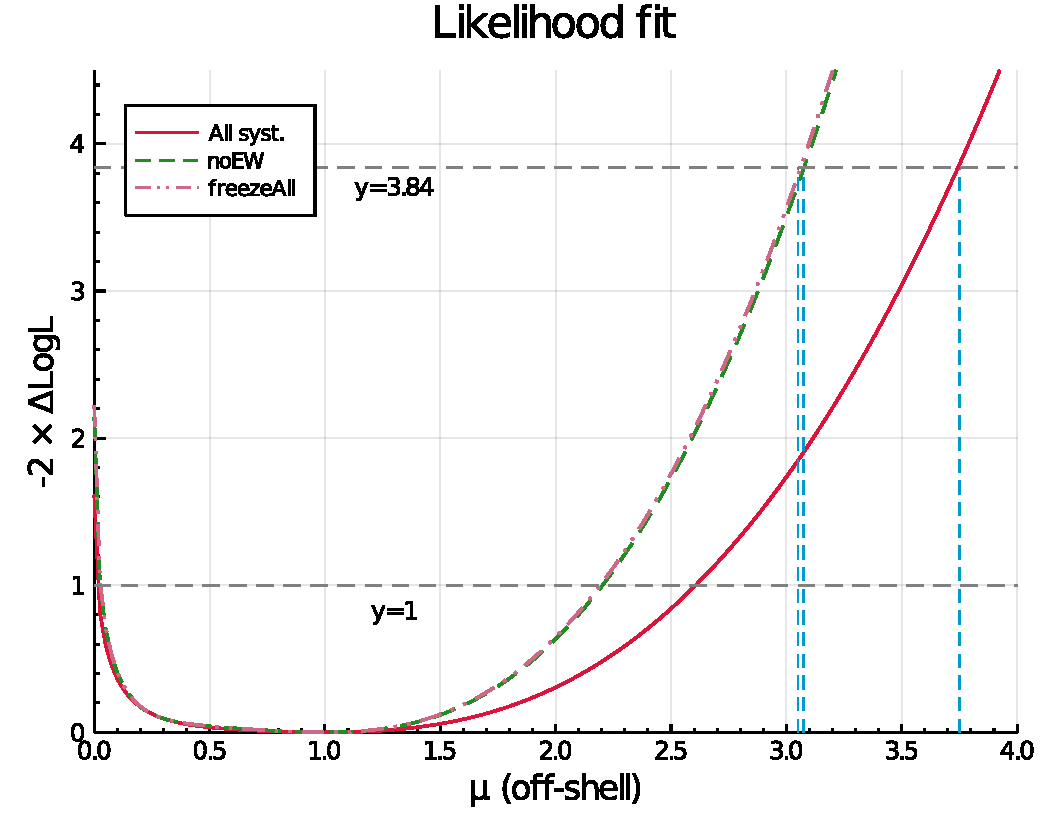
\includegraphics[width=.8\linewidth]{fig/Final_fit_mu_offshell.pdf}
    \caption{Maximum likelihood fit of $\mu^\mathrm{H}_\mathrm{off-shell}$ (off-shell rate ratio).
    For all systematics (red), no Electroweak syst.~(green),
    0 syst.~(orange): y-intersect=\{2.82, 3.49, 3.59\}, 1$\sigma$ lower limits=\{0.075, 0.075, 0.075\},
1$\sigma$ higher limits=\{2.45, 2.13, 2.1\}, 95\% CL limits=\{3.5, 2.9, 2.9\}, respectively.}
    \label{fig:final_fit_mu}
\end{figure}
After running through Combined Limited tool~\cite{combine1, combine2, combine3} for likelihood fitting, we first extract the significance
of the off-shell rate.~(Fig.~\ref{fig:final_fit_mu})
The y-axis is understood to be $\sigma^2$ in terms of significance. Thus
the intersection with the y-axis is the signal sensitivity. In other words,
rejection of the 0 width hypothesis (no off-shell) has a significance of 
$\sqrt{1.61} \approx 1.26\sigma$ in this fit with all the systematic uncertainties included.
As the systematics are `turned off', the constraint becomes tighter, producing an error band for the expected
final result in the upcoming official analysis. The electroweak uncertainty is displayed individually as
it encompasses most of the systematic uncertainties.

\begin{figure}[h]
    \centering
    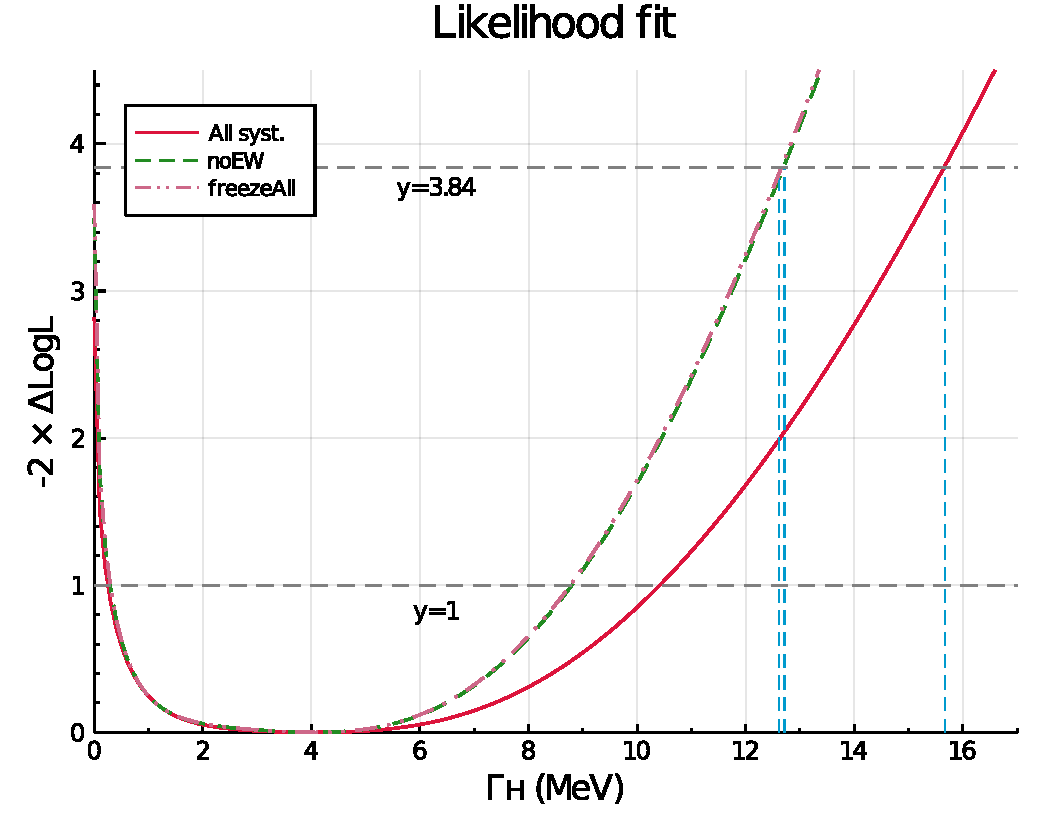
\includegraphics[width=.8\linewidth]{fig/Final_fit_width.pdf}
    \caption{Maximum likelihood fit of Higgs decay width. For all systematics (red), no Electroweak syst.~(green),
    0 syst.~(orange): y-intersect=\{2.82, 3.49, 3.59\}, 1$\sigma$ lower limits=\{0.20, 0.31, 0.31\} MeV,
1$\sigma$ higher limits=\{10.38, 8.75, 8.65\} MeV, 95\% CL limits=\{15.67, 12.72, 12.62\} MeV, respectively.}
\label{fig:final_fit_width}
\end{figure}
Furthermore, by un-constraining the $\mu_\mathrm{F}$ and $\mu_\mathrm{V}$, which are the production rate
of Higgs from fermion fusion vs.\ massive boson fusion as mentioned in the Eqn.~\ref{eqn:diff_xsec}, we can
obtain the limit on the $\Gamma_\mathrm{H}$ itself.
We adopt the range suggested~\cite{rfrv_higgs_pas} for these two systematics. The constraint on the decay width of Higgs $\Gamma_\mathrm{H}$ is shown in 
Fig.~\ref{fig:final_fit_width}. The minimal (max likelihood) falls on \SI{4.07}{\mega\electronvolt},
which is consistent with the standard model hypothesis.
Again, 1$\sigma$ and 95\% CL are marked respectively. And a final result of 
$\Gamma_\mathrm{H}<\SI{16.38}{\mega\electronvolt}$ 95\% CL can be quoted.

% without that, what you are showing is actually off-shell signal strength with the assumption that the ratio 
% of the signal strengths for gg and EW productions are as in the SM.

